%%%%%%%%%
\begin{figure*}
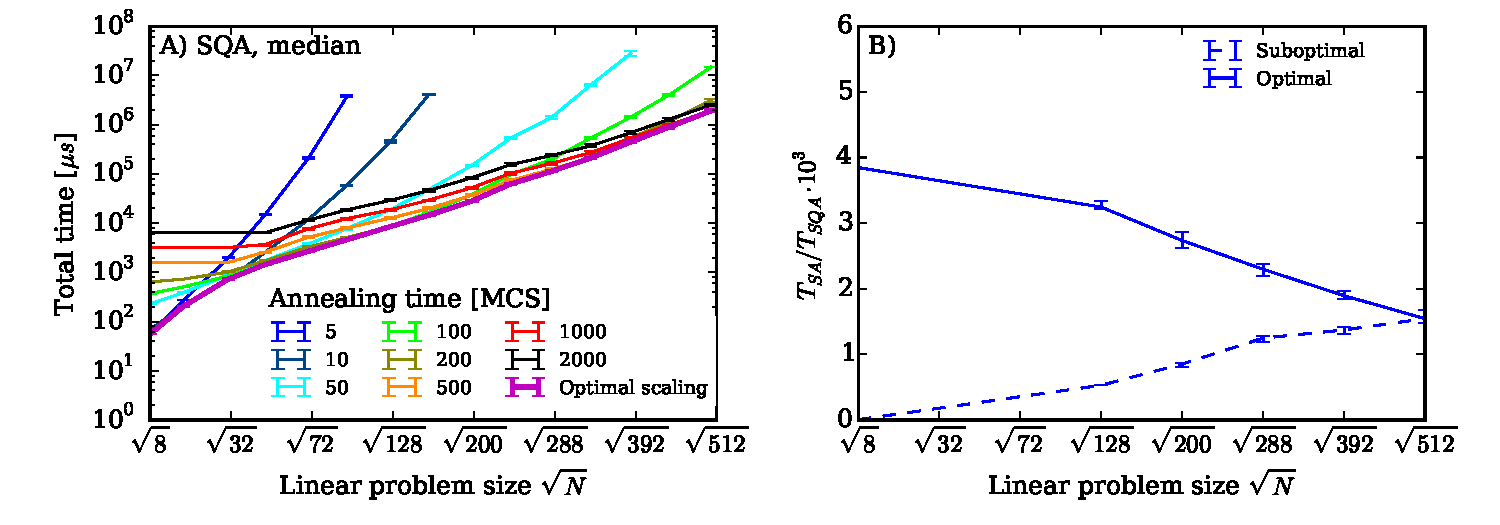
\includegraphics[width=\columnwidth]{fig01.pdf}
\caption{{\bf Pitfalls when detecting speedup.} A) The typical (median)  time to find a ground state at least once with 99\%  probability for spin glasses with $\pm1$ couplings using SQA at constant annealing time. The lower envelope of the curves at constant $t_a$ corresponds to the total effort at an optimal size-dependent annealing time $t_a^{\rm opt}(N)$ and can be used to infer the asymptotic scaling. The initial, relatively flat slope at fixed $N$ is due to suboptimal performance at small problem sizes $N$, and should therefore not be interpreted as speedup. Annealing times are given in units of Monte Carlo steps (MCS), corresponding to one update per spin. B) The speedup of SQA over SA for two cases. If SQA is run suboptimally at small sizes by choosing a fixed large annealing time $t_a=10000$ MCS (dashed line) a speedup is feigned. This is due to suboptimal performance on small sizes and not indicative of the real asymptotic behavior when both codes are run optimally (solid line).}
\label{fig:medianfixed}
\end{figure*}
%%%%%%%%%
